% --------------------------------------------------------------
% This is all preamble stuff that you don't have to worry about.
% Head down to where it says "Start here"
% --------------------------------------------------------------
 
\documentclass[12pt]{article}
 
\usepackage[margin=1in]{geometry} 
\usepackage{amsmath,amsthm,amssymb,scrextend}
\usepackage{fancyhdr}
\usepackage{enumitem}
\usepackage{amsmath}
\usepackage{amssymb}
\usepackage{textcomp}
\usepackage{fancybox}
\usepackage{tikz}
\usepackage{tasks}
\pagestyle{fancy}
\usepackage[makeroom]{cancel}
\usepackage{graphicx}
\usepackage{caption}
\usepackage{mwe}


\usepackage{tikz}
\usetikzlibrary{positioning}

\newenvironment{rcases}
  {\left.\begin{aligned}}
{\end{aligned}\right\rbrace}

\newcommand{\N}{\mathbb{N}}
\newcommand{\Z}{\mathbb{Z}}
\newcommand{\I}{\mathbb{I}}
\newcommand{\R}{\mathbb{R}}
\newcommand{\Q}{\mathbb{Q}}
\renewcommand{\qed}{\hfill$\blacksquare$}
\let\newproof\proof
\renewenvironment{proof}{\begin{addmargin}[1em]{0em}\begin{newproof}}{\end{newproof}\end{addmargin}\qed}
% \newcommand{\expl}[1]{\text{\hfill[#1]}$}
 
\newenvironment{theorem}[2][Theorem]{\begin{trivlist}
\item[\hskip \labelsep {\bfseries #1}\hskip \labelsep {\bfseries #2.}]}{\end{trivlist}}
\newenvironment{lemma}[2][Lemma]{\begin{trivlist}
\item[\hskip \labelsep {\bfseries #1}\hskip \labelsep {\bfseries #2.}]}{\end{trivlist}}
\newenvironment{problem}[2][Problem]{\begin{trivlist}
\item[\hskip \labelsep {\bfseries #1}\hskip \labelsep {\bfseries #2.}]}{\end{trivlist}}
\newenvironment{exercise}[2][Exercise]{\begin{trivlist}
\item[\hskip \labelsep {\bfseries #1}\hskip \labelsep {\bfseries #2.}]}{\end{trivlist}}
\newenvironment{reflection}[2][Reflection]{\begin{trivlist}
\item[\hskip \labelsep {\bfseries #1}\hskip \labelsep {\bfseries #2.}]}{\end{trivlist}}
\newenvironment{proposition}[2][Proposition]{\begin{trivlist}
\item[\hskip \labelsep {\bfseries #1}\hskip \labelsep {\bfseries #2.}]}{\end{trivlist}}
\newenvironment{corollary}[2][Corollary]{\begin{trivlist}
\item[\hskip \labelsep {\bfseries #1}\hskip \labelsep {\bfseries #2.}]}{\end{trivlist}}




\setlength{\parindent}{0pt}
\begin{document}
\setcounter{section}{4}

 \settasks{
	counter-format=(tsk[r]),
	label-width=4ex
}
% --------------------------------------------------------------
%                         Start here
% --------------------------------------------------------------

\lhead{Math 475}
\chead{Chapter 5}
\rhead{Meenmo K.}

\section{Binomial Theorem }
{\sl Goal}: Expand $(x+y)^n$ quickly.

\subsection{Pascal's Triangle}
$$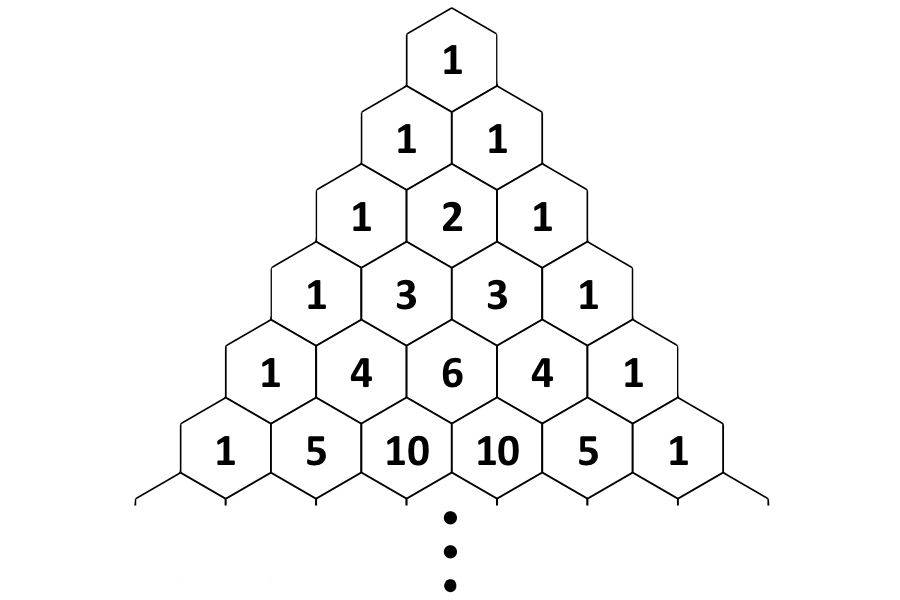
\includegraphics[height=4cm, width=7cm]{pascal.jpg}$$
Each number is the sum of the two above it.

\begin{align*}
    (x+y)^0&=1\\
    (x+y)^1&=x+y\\
    (x+y)^2&=x^2+2xy+y^2\\
    (x+y)^3&=x^3+3x^2y+3xy^2+y^3\\
    (x+y)^4&=(x+y)(x+y)^3\\
           &=(x+y)(x^3+3x^2y+3xy^2+y^3)\\
          &=x^4+3x^3y+3x^2y^2+xy^3+x^3y+3x^2y^2+3xy^3+y^4\\ &=x^4+4x^3y+6x^2y^2+4xy^3+y^4
\end{align*}

\underline{Recall}: Pascal's Formula
$$\binom{n}{k}=\binom{n-1}{k-1}+\binom{n-1}{k}$$
What this tells us is that Pascal's triangle is also 
\begin{center}
    \begin{tabular}{rccccccccc}
&    &    &    &    &  $\binom{0}{0}$\\\noalign{\smallskip\smallskip}
&    &    &    &  $\binom{1}{0}$ &    &  $\binom{1}{1}$ \\\noalign{\smallskip\smallskip}
&    &    &  $\binom{2}{0}$ &    &  $\binom{2}{1}$ &    &  $\binom{2}{2}$\\\noalign{\smallskip\smallskip}
&    &  $\binom{3}{0}$ &    &  $\binom{3}{1}$ &    &  $\binom{3}{2}$ &    &  $\binom{3}{3}$\\\noalign{\smallskip\smallskip}
&  $\binom{4}{0}$ &    &  $\binom{4}{1}$ &    &  $\binom{4}{2}$ &    &  $\binom{4}{3}$ &    &  $\binom{4}{4}$\\\noalign{\smallskip\smallskip}
\end{tabular}
\end{center}

Properties
\begin{itemize}
    \item Pascal's Triangle has vertical reflective symmetry because $\binom{n}{k}=\binom{n}{n-k}$
    
    \item Rows add to $2^n$ because $\sum\limits_{k=0}^n \binom{n}{k} = 2^n$
\end{itemize}

\subsection{Binomial Theorem}
$$(x+y)^n = \sum\limits_{k=0}^n \binom{n}{k}x^{n-k}y^k \left[= \sum\limits_{k=0}^n \binom{n}{k}x^{k}y^{n-k} =
\sum\limits_{k=0}^n \binom{n}{n-k}x^{n-k}y^k =
\sum\limits_{k=0}^n \binom{n}{n-k}x^{k}y^{n-k}\right]$$
{\sl Example} 
\begin{align*}
    (x+y)^6 &= \sum\limits_{k=0}^6\binom{6}{k}x^{6-k}y^k\\
    &=\binom{6}{0}x^6y^0+\binom{6}{1}x^5y^1+\binom{6}{2}x^4y^2+\binom{6}{3}x^3y^3+\binom{6}{4}x^2y^4+\binom{6}{5}x^1y^5+\binom{6}{6}x^0y^6
\end{align*}

\underline{Proof Idea 1}: 
$$(x+y)^n = \underbrace{(x+y)(x+y)\ldots(x+y)}_{\text{$n$ times}}$$

We know this will be a sum of monomials $x^{n-k}y^k$. (The number of x and y equals $n$)\\

The coefficient is the number of ways to choose $x$ (or $y$) at each stage.
i.e.
$$\binom{n}{n-k}=\binom{n}{k}$$

\vspace{1.5\baselineskip}
\underline{Special Case} (Theorem. 5.2.2): Let $y=1$ in binomial theorem.
$$(1+x)^n = \sum\limits_{k=0}^n \binom{n}{k}x^k = \sum\limits_{k=0}^n \binom{n}{n-k}x^k$$

\vspace{1.5\baselineskip}
\subsection{Unimodality of Binomial Coefficients}
Combinatorial Identities

\begin{align}
    k\binom{n}{k} = n\binom{n-1}{k-1} \tag{5.2}\nonumber
\end{align}

\vspace{1.5\baselineskip}
set $x=y=1$ in binomial theorem to get:
\begin{align}
    (1+1)^n = 2^n=\binom{n}{0} +\binom{n}{1} + \ldots +\binom{n}{n} \tag{5.3} \nonumber
\end{align}

\vspace{1.5\baselineskip}
set $x=1$ and $y=-1$ in binomial theorem to get:
\begin{align}
    (1-1)^n &= 2^n=\binom{n}{0}(-1)^1 +\binom{n}{1}(-1)^2 + \ldots +\binom{n}{n}(-1)^n \nonumber\\
    0 &= \binom{n}{0} - \binom{n}{1} + \binom{n}{2}-\binom{n}{3} + \ldots + (-1)^n\binom{n}{n} \tag{5.4} 
\end{align}

Add (5.3) and (5.4)
\begin{align}
    2^n+0 &= \binom{n}{0} + \binom{n}{1} +\binom{n}{2} + \ldots +\binom{n}{n} +\binom{n}{0} - \binom{n}{1} + \binom{n}{2} = \binom{n}{3} + \ldots + (-1)^n\binom{n}{n}\nonumber
\end{align}
\begin{align}
    2^n &=2\binom{n}{0} + 2\binom{n}{2} + 2\binom{n}{4} + \ldots + 2\begin{cases}
    \binom{n}{n-1} &\text{if $n$ odd}\nonumber \\
    \binom{n}{n} &\text{if $n$ even}
    \end{cases}\nonumber\\
    (5.6)\qquad 2^{n-1} &= \binom{n}{0}+\binom{n}{2}+\binom{n}{4}+\ldots\tag{\text{all terms are eventually 0}}\\
    \text{Subtracting 5.4 from 5.3, we get}\nonumber \\
    (5.7)\qquad 2^{n-1} &= \binom{n}{1}+\binom{n}{3} + \binom{n}{5} + \ldots \nonumber \\
    (1+x)^n&=\binom{n}{0}+\binom{n}{1}x+\binom{n}{2}x^2 +\ldots + \binom{n}{n}x^n \nonumber \\
    \text{Differentiate both sides with respect to $x$} \nonumber \\
    n(x+1)^{n-1} &= \binom{n}{1}+2\binom{n}{2}x+3\binom{n}{3}x^2 + \ldots + n\binom{n}{n}x^{n-1} \nonumber \\
    \text{Letting $x=1$, we obtain}\nonumber \\
    n\cdot 2^{n-1} &= \binom{n}{1}+2\binom{n}{2}+3\binom{n}{3}+\ldots + n\binom{n}{n} \tag{5.8}
\end{align}
\begin{align}
    \sum\limtis_{k=0}^n \binom{n}{k}^2 = \binom{2n}{n} \tag{5.16}\\
    \text{are equivalent to}\nonumber \\
    \sum\limits_{k=0}^n \binom{n}{k}\binom{n}{n-k} \nonumber
\end{align}
These count $\binom{2n}{n}$ in 2 different ways, directly and by looking at how many elements are taken from each of two subcollections of $n$ things.

\vspace{1.5\baselineskip}
$\binom{r}{k}$ makes sense if $r$ is a real number and $k$ is any integer. In this case,
$$\binom{r}{k}=\begin{cases}
\frac{r(r-1)(r-2)\ldots(r-k+1)}{k!} & \text{if }k\ge 1\\
1&\text{if } k=0\\
0&\text{if } k=\le -1
\end{cases}$$

\underline{Example} $r=\frac{1}{2},\;k=3$
\begin{align*}
    \binom{\frac{1}{2}}{3} &= \frac{\left(\frac{1}{2}\right)\left(\frac{-1}{2}\right)\left(\frac{-3}{2}\right)}{3!} = \frac{3}{48} = \frac{1}{16} \\
    \binom{\sqrt{2}}{-1} &=0\\
    \binom{4\cdot 8}{0}  &= 1\\
    \binom{-4}{5} &= \frac{(-4)\cdot(-5)\cdot(-6)\cdot(-7)\cdot(-8)}{5!} -56
\end{align*}

It is still true that
\begin{align}
    \binom{r}{k} &= \binom{r-1}{k} + \binom{r-1}{k-1} \tag{Pascal's Formula}\\
    k\binom{r}{k} &= r\binom{r-1}{k-1} \nonumber\\
    \nonumber\\
\text{If $k$ is a positive integer,}\nonumber\\
    \binom{r}{k} &= \binom{r-1}{k} + \binom{r-1}{k-1}\nonumber\\
    &= \binom{r-1}{k} + \binom{r-2}{k-1} + \binom{r-2}{k-2}\nonumber\\
    &=\binom{r-1}{k} + \binom{r-2}{k-1} + \binom{r-3}{k-2} + \binom{r-3}{k-3}\nonumber\nonumber \\
    &= \binom{r-1}{k}+\binom{r-2}{k-1}+\binom{r-3}{k-2}+\ldots+\binom{r-k}{1}+\binom{r-k}{0}\nonumber \\
    &= \binom{r-1}{k}+\binom{r-2}{k-1}+\binom{r-3}{k-2}+\ldots+\binom{r-k}{1}+\binom{r-k-1}{0}+\nonumber \\
    &\qquad\cancel{\binom{r-k-1}{-1}} \nonumber
\end{align}
Replace $r$ with $r+k+1$
\begin{align}
    \binom{r}{0} + \binom{r+1}{1} + \binom{r+2}{2} + \ldots + \binom{r+k}{k}=\binom{r+k+1}{k} \tag{5.18} \\
\end{align}
For $n,\;k$ positive integers,
\begin{align*}
    \binom{n}{k} &= \binom{n-1}{k}+\binom{n-1}{k-1} \\
    &=\binom{n-2}{k} +\binom{n-2}{k-1}+\binom{n-1}{nk-1}\\
    &=\binom{n-3}{k}+\binom{n-3}{k-1}+\binom{n-2}{k-1}+\binom{n-1}{k-1}\\
    \vdots\\
    &=\cancel{\binom{0}{k}} + \cancel{\binom{0}{k-1}}+\binom{1}{k-1}+\ldots+\binom{n-1}{k-1}
\end{align*}

\vspace{1.5\baselineskip}
\subsection{Multinomial Theorem}
Suppose we need to compute $(x+y+z)^3$
\begin{enumerate}
    \item We could multiply it all out. If we are clever, we will automate it with some combinatorial reasoning.
    \item We could use the binomial theorem {\sl twice}.
    \begin{align*}
        (x+(y+z))^3 &= \binom{3}{0}x^3+\binom{3}{1}x^2(y+z)^1 + \binom{3}{2}x(y+z)^2+\binom{3}{3}(y+z)^3 \\
        &= \binom{3}{0}x^3 + \binom{3}{1}\binom{1}{0}x^2y +\binom{3}{1}\binom{1}{1}x^2z+\binom{3}{2\binom{2}0}xy^2+\binom{3}{2}\binom{2}{1}xyz+\\
        &\quad\binom{3}{2}\binom{2}{1}xz^2+\binom{3}{3}\binom{3}{0}y^3+\binom{3}{3}\binom{3}{1}y^2z+\binom{3}{3}\binom{3}{2}yz^2+\binom{3}{3}\binom{3}{3}z^3
    \end{align*}
\end{enumerate}

\vspace{1.5\baselineskip}
\underline{Notation}: $$\underbrace{\binom{n}{n_1\;n_2\;n_3\ldots n_t}}_{\text{$n_i$ is multinomial coefficient}} = \frac{n!}{n_1!\;n_2!\;n_3!\ldots n_t!}$$
This refers to the number of ways to arrange $n$ objects that include 
\begin{itemize}
    \item[] $n_1$ identical objects
    \item[] $n_2$ identical objects
    \item[] \qquad\qquad\vdots
    \item[] $n_t$ identical objects
\end{itemize}
Note that $\sum\limits_{n=1}^t=n$.

\vspace{1.5\baselineskip}
{\sl Example} Permutation of WISCONSIN
$$\binom{9}{1\; 2\;2\;1\;1\;2}=\frac{9!}{1!2!2!1!1!2!}$$

\vspace{1.5\baselineskip}
Note that $$\binom{n}{k} = \binom{n}{k(n-k)}$$\\
Also
$$\binom{n}{n_1n_2\ldots n_t} = \binom{n}{n_1}\binom{n-n_1}{n_2}\binom{n-n_1-n_2}{n_3}\ldots\binom{n-n_1-n_2-\ldots-n_{t-1}}{n_t}$$

\vspace{1.5\baselineskip}
{\bf Multinomial Theorem}\\
{\sl Example}
\begin{align*}
    (x+y+z)^3 &= (x+y+z)(x+y+z)(x+y+z)\\
    &=\binom{3}{3}x^3+\binom{3}{2\;1}x^2y+\binom{3}{1\;2}xy^2 +\binom{3}{3}y^3+\binom{3}{2\;1}x^2z+\binom{3}{1\;2}xz^2 +\\
    &\quad\binom{3}{1\;1\;1}xyz+\binom{3}{2\;1}y^2z+\binom{3}{1\;2}yz^2 + \binom{3}{3}z^3
\end{align*}

{\bf Theorem 5.4.1 Multinomial Theorem}\\
\begin{align*}
    (x_1+x_2+x_3+...+x_t)^n &= \sum\binom{n}{n_1n_2\ldots n_t}x_1^{n_1}x_2^{n_2}x_3^{n_3}\ldots x_t^{n^t}
\end{align*}

where the sum is over all non-negative integers $n_1,\;n_2,\;...,\;n_t$ such that $n_1+n_2+...+n_t=n$.\\

{\sl Example} Find the coefficient of $x^4y^3z^2w$ in $(x+y+z+w)^{10}$.
$$\binom{10}{4\;3\;2\;1}=\frac{10!}{4!3!2!1!}$$\\

{\sl Example} Find the coefficient of $x^4y^3z^2w^$ in $(x+y+z+w)^{10}$\\

It is 0 because 4+3+2+2=11, so there is no such term.\\

{\sl Pascal's Formula}\\
$$\binom{n}{n_1\;n_2\;\ldots\;n_t} = \binom{n-1}{n_1-1\;n_2\ldots n_t}+\binom{n-1}{n_1\;n_2-1\ldots n_t}+\ldots+\binom{n-1}{n_1\;n_2\ldots n_t-1}$$\\

\subsection{Newton's Extended Binomial Theorem}
\begin{align}
    (x+y)^\alpha = \sum\limits_{k=0}^\infty\binom{\alpha}{k}x^ky^{\alpha-y} \tag{for any real number $\alpha$}
\end{align}

{\sl Special Case} Let $z$ be a complex number with $|z|<1$. Then
$$(1+z)^\alpha = \sum\limits{k=0}^\infty\binom{\alpha}{k}z^k$$\\

{\sl Example}: $\alpha=3$
\begin{align*}
    (1+z)^3 &= \sum\limits{k=0}^\infty\binom{3}{k}z^k = \binom{3}{0} + \binom{3}{1}z + \binom{3}{2}z^2 +\binom{3}{3}z^3 + \binom{3}{4}z^4+...\\
    &=1+3z+3z^2+z^3+0+...\\
    &=1+3z+3z^2+z^3
\end{align*}

\vspace{1.5\baselineskip}
{\sl Example}: $\alpha=-1$
\begin{align*}
    (1+z)^{-1} &= \sum\limits_{k=0}^\infty\binom{-1}{k}z^k = \binom{-1}{0} + \binom{-1}{1}z+\binom{-1}{2}z^2 + \binom{-1}{3}z^3+\ldots\\
    &=1-z+z^2-z^3+z^4-...\\
\end{align*}

This is just the sum of an infinite geometric series in disguise.
   $$ \frac{1}{1-z}&=1+z+z^2+z^3+...$$
\begin{align*}
    \binom{-1}{k} &= \frac{(-1)(-1-1)(-1-2)\ldots(-1-(k-1))}{k!}\\
    &=\frac{(-1)(-2)(-3)\ldots(-k)}{k!} = (-1)^k\cdot \frac{k!}{k!} = (-1)^k
\end{align*}

\underline{Recall}: $(1-x)^{-1} = 1+x+x^2+x^3+\dotsb$\\

By Newton's Extended Binomial Theorem,
\begin{align*}
    (1-x)^{-n} &= \sum\limits_{k=0}^\infty \binom{-n}{k}(-x)^k \\
    &=\binom{-n}{0}(-x)^0+\binom{-n}{1}(-x)^1+\binom{-n}{2}(-x)^2+\binom{-n}{3}(-x)^3+\dotsb\\
     &=1+\frac{(-n)}{1!}(-x)+\frac{(-n)(-n-1)}{2!}x^2+\frac{(-n)(-n-1)(-n-2)}{3!}(-x^3)+\dotsb \\
    &=1+\binom{n}{1}x+\frac{(n+1)!}{2!(n-1)!}x^2+\frac{(n+2)!}{3!(n-1)!}x^3+\dotsb+\frac{(n+r-1)!}{r!(n-1)!}x^r+\dotsb\\
    &=1+\binom{n}{1}x+\frac{(n+1)!}{2!(n-1)!}x^2+\frac{(n+2)!}{3!(n-1)!}x^3+\ldotsb+\frac{(n+r-1)!}{r!(n-1)!}x^r+\dotsb\\
    &=1+\binom{n}{1}x+\binom{n+1}{2}x^2+\binom{n+2}{3}x^3+\dotsb+\binom{n+r-1}{r}x^r+\dotsb\\
    (1-x)^{-n}&=\sum\limits_{r=0}^\infty\binom{n+r-1}{r}x^r\\
    &=(1+x+x^2+\dotsb)^n \\
    &= \underbrace{(1+x+x^2+\dotsb)(1+x+x^2+\dotsb)\dotsb(1+x+x^2+\dotsb)}_{n\;times}\\
\end{align*}

\begin{align*}
    \sqrt{1+x} =(1_x)^{1/2} &=\sum\limits_{k=0}^\infty\binom{1/2}{k}x^k\\
    &=\binom{1/2}{0}+\binom{1/2}{1}x+\binom{1/2}{2}x^2+\binom{1/2}{3}x^3+\dotsb+\binom{1/3}{r}x^r+\dotsb\\
    &=1+\frac{\left(\frac{1}{2}\right)}{1!}
    +\frac{\left(\frac{1}{2}\right)\left(\frac{1}{2}\right)}{2!}x^2+\frac{\left(\frac{1}{2}\right)\left(\frac{-1}{2}\right)\left(\frac{1}{2}\right)}{3!}x^3+\dotsb+\frac{\left(\frac{1}{2}\right)\left(\frac{-1}{2}\right)\dotsb\left(\frac{1}{2}-r+1\right)}{r!}x^r+\dotsb\\
    &=1+\frac{1}{2}x-\frac{1}{8}x^2+\frac{1}{16}x^3+\dotsb+\frac{(-1)^{r-1}}{r\cdot2^{2r-1}}\binom{2r-2}{r-1}x^r+\dotsb\\
    &=\sum\limits_{k=0}^\infty\frac{(-1)^{k-1}}{k\cdot 2^{2k-1}}\binom{2k-2}{k-1}x^k
\end{align*}

\newpage
{\sl Example:} Estimate $\sqrt{20}$\\
We could treat this as $\sqrt{1+19}$, but we need to have $|x|<1$ for a good estimate.
\begin{align*}
    \sqrt{20} &= \sqrt{16+4} &= \sqrt{16}\left(\sqrt{1+\frac{1}{4}}\right) &=4\sqrt{1+\frac{1}{4}}\\
    &&&\approx 4\left(1+\frac{1}{2}-\frac{1}{8}\left(\frac{1}{4}\right)^2+\frac{1}{16}\left(\frac{1}{4}\right)^3\right)\\
    &&&=\left(1+\frac{1}{8}-\frac{1}{128}+\frac{1}{1024}\right)\\
    &&&=4.472
\end{align*}






\end{document}
